\documentclass[11pt,ignorenonframetext,compress]{beamer}
\setbeamertemplate{caption}[numbered]
\setbeamertemplate{caption label separator}{: }
\setbeamercolor{caption name}{fg=normal text.fg}
\beamertemplatenavigationsymbolsempty
\usepackage{lmodern}
\usepackage{amssymb,amsmath}
\usepackage{natbib}
\usepackage{booktabs}
\usepackage{ifxetex,ifluatex}
\usepackage{fixltx2e} % provides \textsubscript
\ifnum 0\ifxetex 1\fi\ifluatex 1\fi=0 % if pdftex
\usepackage[T1]{fontenc}
\usepackage[utf8]{inputenc}
\else % if luatex or xelatex
\ifxetex
\usepackage{mathspec}
\else
\usepackage{fontspec}
\fi
\defaultfontfeatures{Ligatures=TeX,Scale=MatchLowercase}
\fi
\usetheme[]{metropolis}
% use upquote if available, for straight quotes in verbatim environments
\IfFileExists{upquote.sty}{\usepackage{upquote}}{}
% use microtype if available
\IfFileExists{microtype.sty}{%
  \usepackage{microtype}
  \UseMicrotypeSet[protrusion]{basicmath} % disable protrusion for tt fonts
}{}
\newif\ifbibliography
\hypersetup{
  pdftitle={Feature-based time series generation and forecasting},
  pdfauthor={with Yanfei Kang and Rob Hyndman},
  pdfborder={0 0 0},
  breaklinks=true}
\urlstyle{same}  % don't use monospace font for urls
\usepackage{graphicx,grffile}
\makeatletter
\def\maxwidth{\ifdim\Gin@nat@width>\linewidth\linewidth\else\Gin@nat@width\fi}
\def\maxheight{\ifdim\Gin@nat@height>\textheight0.8\textheight\else\Gin@nat@height\fi}
\makeatother
% Scale images if necessary, so that they will not overflow the page
% margins by default, and it is still possible to overwrite the defaults
% using explicit options in \includegraphics[width, height, ...]{}
\setkeys{Gin}{width=\maxwidth,height=\maxheight,keepaspectratio}

% Prevent slide breaks in the middle of a paragraph:
\widowpenalties 1 10000
\raggedbottom

\AtBeginPart{
  \let\insertpartnumber\relax
  \let\partname\relax
  \frame{\partpage}
}
\AtBeginSection{
  \ifbibliography
  \else
  \let\insertsectionnumber\relax
  \let\sectionname\relax
  \frame{\sectionpage}
  \fi
}
\AtBeginSubsection{
  \let\insertsubsectionnumber\relax
  \let\subsectionname\relax
  \frame{\subsectionpage}
}

\setlength{\parindent}{0pt}
\setlength{\parskip}{6pt plus 2pt minus 1pt}
\setlength{\emergencystretch}{3em}  % prevent overfull lines
\providecommand{\tightlist}{%
  \setlength{\itemsep}{0pt}\setlength{\parskip}{0pt}}
\setcounter{secnumdepth}{0}
%% header.tex
%%
%% Copyright (C) 2016 - 2017  Dirk Eddelbuettel
%%
%% This file is part of samples-rmarkdown-metropolis repository.
%%
%% samples-rmarkdown-metropolis is free software: you can redistribute it
%% and/or modify it under the terms of the GNU General Public License as
%% published by the Free Software Foundation, either version 2 of the
%% License, or (at your option) any later version.
%%
%% samples-rmarkdown-metropolis is distributed in the hope that it will be
%% useful, but WITHOUT ANY WARRANTY; without even the implied warranty of
%% MERCHANTABILITY or FITNESS FOR A PARTICULAR PURPOSE.  See the GNU General
%% Public License for more details.
%%
%% You should have received a copy of the GNU General Public License along with
%% samples-rmarkdown-metropolis.  If not, see <http://www.gnu.org/licenses/>.

%% If you have the Fira font installed, to actually have it used it
%% via rmarkdown you need to declare it here
% \setsansfont[ItalicFont={Fira Sans Light Italic},BoldFont={Fira Sans},BoldItalicFont={Fira Sans Italic}]{Fira Sans Light}
% \setmonofont[BoldFont={Fira Mono Medium}]{Fira Mono}
% \usepackage[orientation=landscape,size=custom,width=16,height=9,scale=0.5,debug]{beamerposter}
\setbeamertemplate{footline}[frame number]
%% You can set various Metropolis options via \metroset{} here
% \metroset{....}
%% You can redefine colours, mostly by borrowing from Beamer
\setbeamercolor{frametitle}{bg=purple}

%% You also use hyperref, and pick colors
\hypersetup{colorlinks,citecolor=purple,filecolor=red,linkcolor=brown,urlcolor=blue}
%% when rendered with rmarkdown, somehow the unicode char for the dot
%% disappears so we redefine it here -- that is an older comments, seems font-specific
%% \renewcommand{\textbullet}{$\cdot$}
%% \renewcommand{\itemBullet}{▸}   % unicode U+25b8 'black right pointing small triangle'

%% The institute macro puts a small line for affiliation at the bottom
\institute{}

%% We can also place a logo
%% \titlegraphic{\hfill\includegraphics[height=1cm]{figures/buaalogo.jpg}}

%%% Local Variables:
%%% mode: latex
%%% TeX-master: t
%%% End:

\title{Feature-based time series generation and forecasting}
\subtitle{Feng Li\\ Central University of Finance and Economics\\\texttt{\url{http://feng.li/}}}
%\author{with Yanfei Kang (Beihang U.) and Rob Hyndman (Monash U.)}
\author{{\em --- based on a series of working papers:}\\ {\footnotesize
    $\ast$  {\color{blue} Efficient generation of time series with diverse and controllable characteristics}\\
    (with Yanfei Kang and Rob Hyndman)\\
    $\ast$ {\color{blue} Forecasting using time series feature spaces}\\
     (with Yanfei Kang and Rob J. Hyndman)\\
    $\ast$ {\color{blue} Time series forecasting based on automatic feature extraction}\\
     (with Yanfei Kang,  Xixi Li)}}
}

\date{}

\begin{document}
\frame{\titlepage}

\section{Motivation}\label{motivation}

\begin{frame}{Motivation}

  \begin{itemize}
  \item Train a time series model (\emph{machine learning with dependent data}) is usually
    costly.

  \item New algorithms are developed every day.

  \centerline{\includegraphics[height=0.3\textheight]{figures/motivation}}


  \item Why not cloud computing? Privacy is the main concern in practice.

  \item A well trained model with my dataset does not necessary work well for your dataset. Why?

  \item Is there an efficient way to \textbf{forecast which algorithm works the best} for
    a particular time series.

  \end{itemize}


\end{frame}

\begin{frame}{The No-Free-Lunch theorem}

  \begin{itemize}
  \item
    There is \textbf{never} universally best method that fits in all situations
    \citep{wolpert1996lack}.
  \item
    The \textbf{explosion of new algorithms} development makes the question even
    more worth focusing.
  \item
    No single forecasting method stands out the best for any type of time
    series \citep{adam1973individual}.
  \end{itemize}


\end{frame}

\section{Literature}\label{literature}

\begin{frame}{Literature}

  \begin{itemize}
  \item
    Features of time series \(\rightarrow\) benefits in producing more
    accurate forecasting accuracies \citep{adam1973individual}.

  \item Features \(\rightarrow\) forecasting method selection rules
    \citep{meade2000evidence}.

  \item
    ``Horses for courses'' \(\rightarrow\) effects of time series features
    to the forecasting performances \citep{Petropoulos2014}.

  \item We could visualize the performances of different forecasting methods in a 2D space
    \(\rightarrow\) to get better understanding of their relative performances
    \citep{kang2017visualising}.

  \end{itemize}

\end{frame}

\begin{frame}{Existing problems}

  \begin{itemize}
    \tightlist
  \item For a collection of time series, a selection process can hardly beat
    \textbf{single-method} forecasting strategies.

    \begin{itemize}
      \tightlist
    \item
      select a good, but not necessarily the best method \citep{meade2000evidence}.
    \item
      impossible to identify one single optimal method based on features
      \citep{Petropoulos2014}.
    \item
      space can not be separated nicely according to the strengths and
      weaknesses of forecasting methods \citep{kang2017visualising}.
    \end{itemize}

\item Possible reasons?

  \begin{itemize}
  \item
    Inadequate time series features
  \item
    limited training time series data (not only in number, but in
    diversity)
  \end{itemize}
\end{itemize}
\end{frame}

\section{What we do?}\label{what-we-do}

\begin{frame}{The framework}

  \centerline{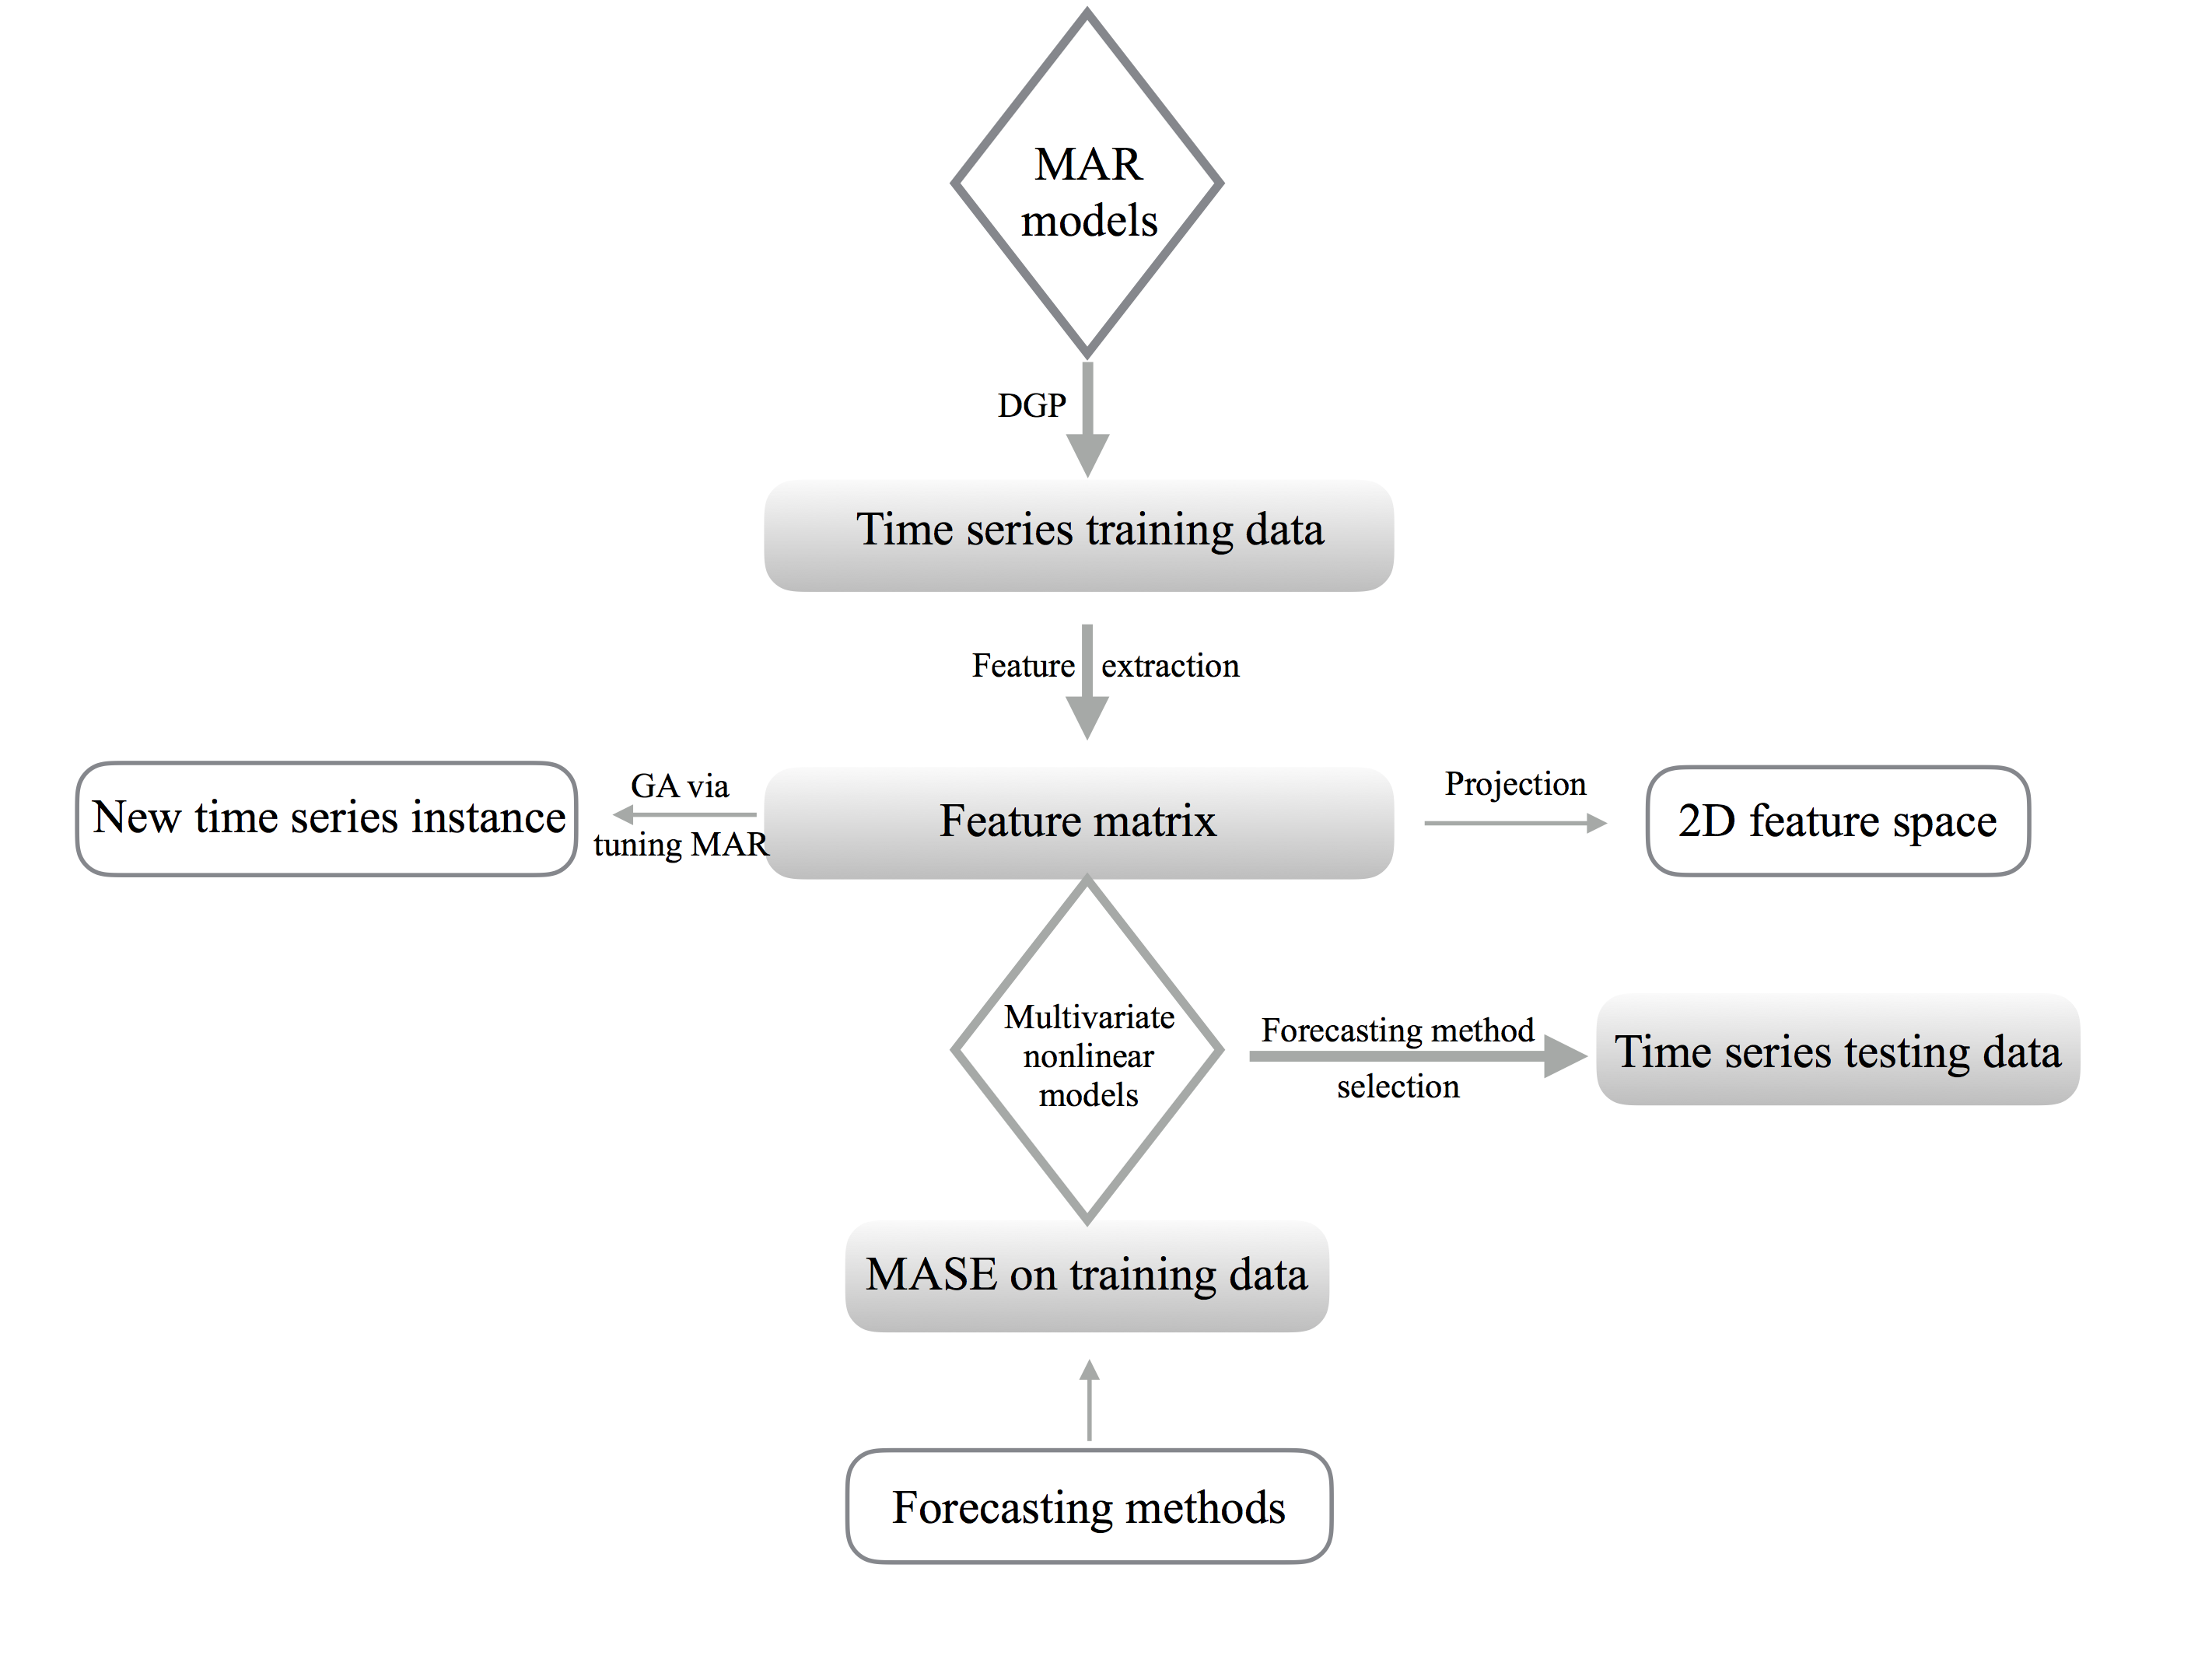
\includegraphics[height=\textheight]{figures/framework.pdf}}

\end{frame}

\begin{frame}{Final aim: forecasting on testing data}

  \begin{itemize}

  \item \textbf{Training data}: Randomly generated data via our DGP procedure.

  \item \textbf{Testing data}: M3 data \citep{makridakis2000m3}

    \begin{itemize}
      \tightlist
    \item
      3003 time series
    \item
      From demography, finance, business and economics
    \item
      Lengths between 14 and 126
    \item
      Either non-seasonal, monthly or quarterly
    \item
      Positive
    \end{itemize}

  \end{itemize}
\end{frame}

% \begin{frame}{Questions to be answered}

%   \begin{itemize}
%     \tightlist
%   \item
%     What time series features?
%   \item
%     How to construct time series training data?
%   \item
%     2D projection?
%   \item
%     How to model features and forecasting methods?
%   \item
%     How to generate new time series with certain features?
%   \end{itemize}

% \end{frame}

\section{Time series features}\label{time-series-features}

\begin{frame}{Basic idea}

  Transform a given time series \(\{x_1, x_2, \cdots, x_n\}\) to a feature
  vector \(F = (F_1, F_2, \cdots, F_p)'\) \citep{kang2017visualising,cikm2015}

  \begin{block}{A feature \(F_k\) can be any kind of function computed
      from a time series:}

    \begin{enumerate}
      \def\labelenumi{\arabic{enumi}.}
      \tightlist
    \item
      A simple mean
    \item
      The parameter of a fitted model
    \item
      Some statistic intended to highlight an attribute of the data
    \item
      \ldots{}
    \end{enumerate}

  \end{block}

\end{frame}

\begin{frame}{Which features should we use?}

  \begin{itemize}
  \item
    There does not exist the best feature representation of a time series
    \citep{fulcher2018feature}.
  \item
    Depends on both the \textbf{nature} of the time series being analysed,
    and the \textbf{purpose} of the analysis.

    \begin{itemize}
    \item
      With unit roots, the mean is not a meaningful feature without some
      constraints on the initial values.
    \item
      CPU usage every minute for a large number of servers: we observe a
      daily seasonality. The mean may provide useful comparative
      information despite the time series not being stationary.
    \end{itemize}
  \end{itemize}

\end{frame}

\begin{frame}{Which features should we use?}

  \begin{itemize}
    \tightlist
  \item
    Time series are of different lengths, on different scales, and with
    different properties.
  \item
    We restrict our features to be ergodic, stationary and independent of
    scale.
  \item
    17 sets of diverse features.
  \item
    New features are intended to measure attributes associated with
    multiple seasonality, non-stationarity and heterogeneity of the time
    series.
  \end{itemize}

\end{frame}


\begin{frame}{Which features should we use?}

  \begin{itemize}
  \item Or automatic feature extraction

    \begin{itemize}
    \item We introduce an automated approach to extract time series features based on
      images
    \item Time series are first transformed into recurrence images, from which local
      features can be extracted using computer vision algorithms.
    \item The extracted features are used for forecast model selection and model
      averaging.
    \end{itemize}

  \end{itemize}

\end{frame}

\begin{frame}{Multiple seasonal time series}

  \begin{figure}
    \centering
    \includegraphics{SH180613_files/figure-beamer/cashdata-1.pdf}
    \caption{Daily cash money demand at some automatic teller machine.}
  \end{figure}

\end{frame}

\begin{frame}{Features for multiple seasonal time series}

  \begin{block}{STL decompostion extension}

    \[ x_t = f_t + s_{1,t} + s_{2,t} + \cdots + s_{M,t} + e_t.\] The
    strength of trend can be measured by: \[
      F_{10} = 1- \frac{\text{var}(e_t)}{\text{var}(f_t + e_t)}.
    \]

    The strength of seasonality for the \(i\)th seasonal component:

    \[
      F_{11,i} = 1- \frac{\text{var}(e_t)}{\text{var}(s_{i,t} + e_t)}.
    \]

  \end{block}

\end{frame}

\begin{frame}{Features on heterogenity}

  \begin{enumerate}
    \def\labelenumi{\arabic{enumi}.}
    \tightlist
  \item
    Pre-whiten the time series \(x_t\) to remove the mean, trend, and
    Autoregressive (AR) information.
  \item
    Fit an GARCH(1,1) model on the pre-whitened time series \(y_t\) to
    measure for the ARCH effects.
  \item
    Test for the arch effects in the obtained residuals \(z_t\) using a
    second GARCH(1,1) model.
  \end{enumerate}

\end{frame}

\begin{frame}{Features on heterogenity}

  \metroset{block=fill}

  \begin{alertblock}{The features of time series on heterogenity.}
    \begin{enumerate}
    \item The sum of squares of the first 12 autocorrelations of $\{y_t^2\}$.
    \item The sum of squares of the first 12 autocorrelations of $\{z_t^2\}$.
    \item The $R^2$ value of an AR model applied to $\{y_t^2\}$.
    \item The $R^2$ value of an AR model applied to $\{z_t^2\}$.
    \end{enumerate}
  \end{alertblock}

\end{frame}

\begin{frame}{Time series features we use}

  \begin{table}[!h]

    % \caption{\label{tab:featuresapp}The features we use to characterize a time series.}
    \centering
    \resizebox{\linewidth}{!}{
      \begin{tabular}[t]{llll}
        \toprule
        \bf Feature & \bf Description & \bf Feature & \bf Description\\
        \midrule
        $F_{1}$ & Number of seasonal periods & $F_{10}$ & Strength of trend\\
        $F_{2}$ & Vector of seasonal periods & $F_{11}$ & Strength of seasonality\\
        $F_{3}$ & Number of differences for stationarity & $F_{12}$ & Spikiness\\
        $F_{4}$ & Number of seasonal differences for stationarity & $F_{13}$ & Autocorrelation coefficients of remainder\\
        $F_{5}$ & Autocorrelation coefficients & $F_{14}$ & ARCH ACF statistic\\
        $F_{6}$ & Partial autocorrelation coefficients & $F_{15}$ & GARCH ACF statistic\\
        $F_{7}$ & Spectral entropy & $F_{16}$ & ARCH $R^2$ statistic\\
        $F_{8}$ & Nonlinearity coefficient & $F_{17}$ & GARCH $R^2$ statistic\\
        $F_{9}$ & Long-memory coefficient &  & \\
        \bottomrule
      \end{tabular}}
  \end{table}


  \begin{itemize}
  \item R package: {\color{blue}\texttt{tsfeatures}} {\footnotesize available on GitHub \url{https://github.com/robjhyndman/tsfeatures}}
  \end{itemize}

  %% \centerline{\includegraphics[width=1.1\textwidth]{figures/tsfeatures.pdf}}

\end{frame}

\begin{frame}[fragile]{A multi-seasonal time series with extracted features}

  \fontsize{7}{8}\sf
  \includegraphics{SH180613_files/figure-beamer/cashfeatures-1.pdf}

  \resizebox{\textwidth}{!}{
    \begin{tabular}{rrrrrr}
      \toprule
      entropy &  x.acf1&  x.acf10&  diff1.acf1& diff1.acf10& diff2.acf1\\
      0.7647817 &0.517701& 1.305203& -0.03341881&   0.6712913& -0.4276741\\
      \midrule
      diff2.acf10& seas.acf1&   x.pacf5& diff1x.pacf5& diff2x.pacf5&  seas.pacf\\
      0.4801166& 0.1024061& 0.4219687&    0.5021309&    0.5093377& 0.01495473\\
      \midrule
      nperiods& seasonal.period1& seasonal.period2&     trend&        spike&\\
      2&                7&              365& 0.6505438& 1.094574e-07&\\
      \midrule
      linearity& curvature&    e.acf1&    e.acf10& seasonal.strength1 &  seasonal.strength2\\
      12.2213&  1.430082& 0.2235961& 0.07897381&          0.8365591 & 0.6138975\\
      \midrule
      peak1& peak2& trough1& trough2& ndiffs& nsdiffs\\
      3&   357&       7&     359&      1&       1 \\
      \midrule
      hurst& nonlinearity&  arch.acf&  garch.acf&   arch.r2&   garch.r2\\
      0.8418821&     0.122436& 0.3669286& 0.02484353& 0.2535115& 0.02558531\\
      \bottomrule
    \end{tabular}
  }
\end{frame}

\section{Training data simulation}\label{training-data-simulation}

\begin{frame}{Gaussian Mixure Autoregressive (MAR) models}

  \begin{itemize}
    \tightlist
  \item
    Consist of multiple stationary or non-stationary autoregressive
    components.\\
  \item
    A \(K\)-component MAR model is defined as \citep{wong2000mixture} : \[
      F(x_t|\mathcal{F}_{t-1}) =
      \sum\limits_{k=1}^K\alpha_k\Phi(\frac{x_t-\phi_{k0}-\phi_{k1}x_{t-1}-\cdots
        -\phi_{kp_k}x_{t-p_k}}{\sigma_k}),
    \] where \(F(x_t|\mathcal{F}_{t-1})\) is the conditional cumulative
    distribution of \(x_t\) give the past information
    \(\mathcal{F}_{t-1}\). \(\Phi(\cdot)\) is the cumulative distribution
    function of the standard normal distribution.
    \(\sum_{k=1}^K \alpha_k= 1\), where \(\alpha_k > 0\),
    \(k = 1, 2, \cdots, K\).
  \end{itemize}

\end{frame}

\begin{frame}{Conditional mean and variance}

  \begin{align*}
    E(x_t|\mathcal{F}_{t-1}) &= \sum\limits_{k=1}^K\alpha_k \mu_{k, t}\\
    \mathrm{var}(x_t|\mathcal{F}_{t-1}) &= \sum\limits_{k=1}^K\alpha_k \sigma_k^2 +
                                          \sum\limits_{k=1}^K\alpha_k \mu_{k, t}^2 - \left(\sum\limits_{k=1}^K\alpha_k
                                          \mu_{k, t}\right)^2.
  \end{align*}

  \begin{itemize}
    \tightlist
  \item
    \(\mathrm{var}(x_t|\mathcal{F}_{t-1})\) changes with conditional means
    of different components.
  \item
    The shape of the conditional distributions of the time series changes
    with time.
  \item
    The MAR models can handle heteroscedasticity, which is common in
    financial time series.
  \end{itemize}

\end{frame}

\begin{frame}{Why MAR models}

  \begin{itemize}
    \tightlist
  \item
    Mixtures of stationary and non-stationary components can yield a
    stationary process.
  \item
    To handle non-stationary time series, one can just include a unit root
    in each component.
  \item
    Possible to capture more (or any) time series features, since
    different specifications of finite mixtures have been shown to be able
    to approximate large nonparametric classes of conditional multivariate
    densities \citep{jiang1999on, li2010flexible, norets2010approximation}.
  \end{itemize}

\end{frame}

\begin{frame}{Simulation settings}

  \centerline{\includegraphics[height=\textheight]{figures/simSettings.pdf}}

\end{frame}

\begin{frame}{Projection and visualisation in 2D space}

  \begin{block}{t-Stochastic Neighbor Embedding (t-SNE)}

    \begin{itemize}
      \tightlist
    \item
      Main idea: convert the distances to conditional probabilities and
      minimize the mismatch (kullback-Leibler divergence) between
      probabilities before and after the mapping.

    \item Nonlinear, and retaining both local and global structure
      \citep{maaten2008visualizing,van2014accelerating}.
    \end{itemize}

  \end{block}

  \begin{block}{PCA}

    \begin{itemize}
      \tightlist
    \item
      Linear, and putting more emphasize on keeping dissimilar data points
      far apart
    \end{itemize}

  \end{block}

\end{frame}

\begin{frame}{Investigating the coverage of MAR models}

  \centerline{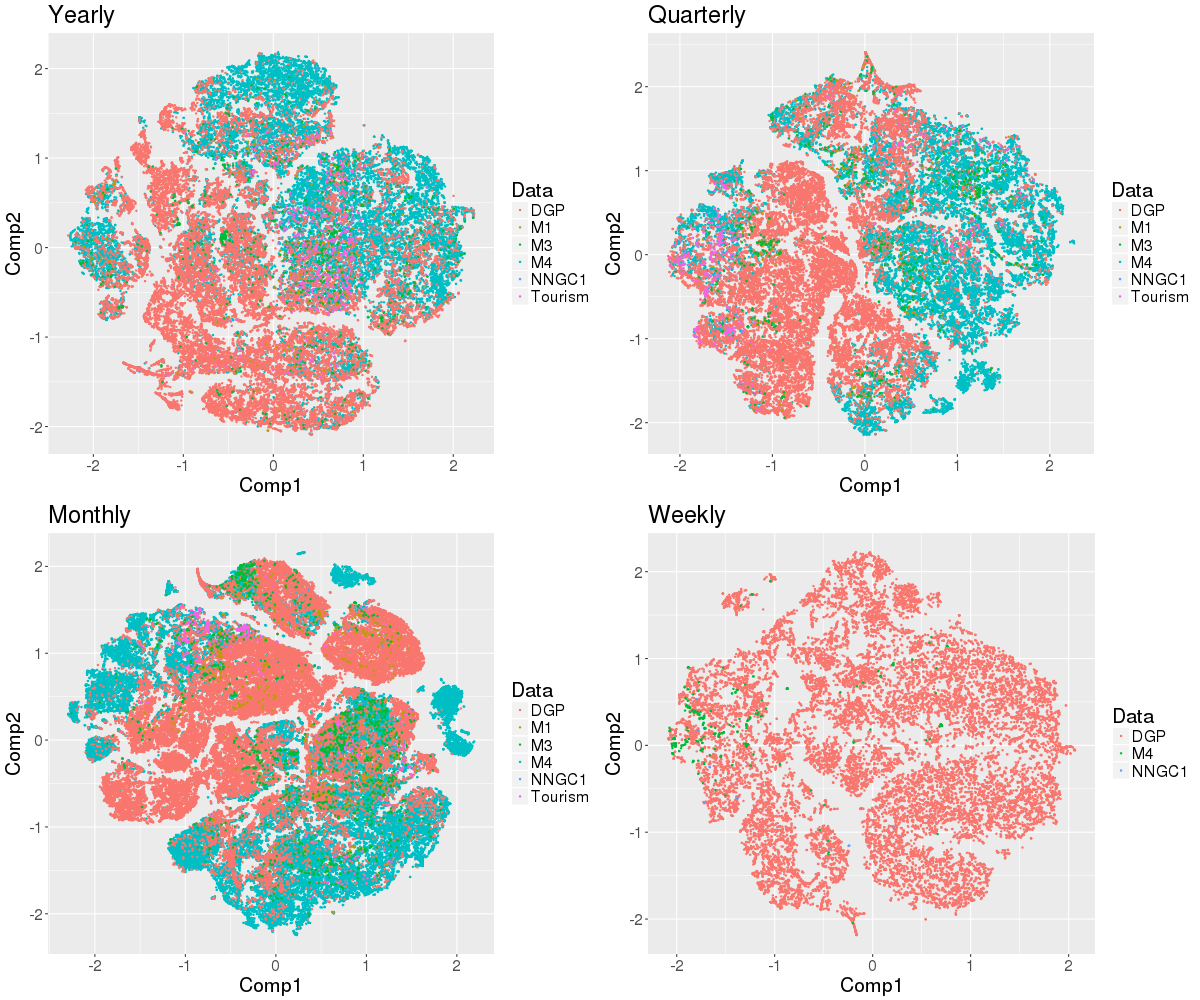
\includegraphics[width=0.9\textwidth]{figures/coverage.png}}

\end{frame}

\begin{frame}{Miscoverage}

  We define the miscoverage of dataset A over dataset B as:

  \begin{itemize}
    \def\labelenumi{\arabic{enumi}.}
    \tightlist
  \item
    Find the maximum ranges of the \(x\) and \(y\) axes reached by the two
    datasets A and B, and cut the \(x\) and \(y\) dimensions into
    \(N_b = 30\) bins.
  \item
    In the constructed two-dimensional grid with \(N_b^2 = 900\) subgrids,
    we denote \(\mathcal{I}_{i,A} = 0\) if no points in dataset A fall
    into the \(i\)th subgrid. \(\mathcal{I}_{i,A} = 1\) otherwise. The
    same defination of \(\mathcal{I}_{i,B}\) applies for dataset B.
  \item
    The miscoverage of dataset A over dataset B is defined as
    \[\text{miscoverage}_{A/B} = \frac{\sum\limits_{i = 1}^{N_b}[(1 - \mathcal{I}_{i,A})*\mathcal{I}_{i,B}]}{N_b^2}.\]
  \end{itemize}

\end{frame}

\begin{frame}{Miscoverage}

  \begin{table}[!thb]
    \centering
    \resizebox{0.55\textwidth}{!}{
      \begin{tabular}{p{2cm}p{1.5cm}p{1.5cm}p{1.5cm}p{1.5cm}p{1.5cm}p{1.5cm}}
        \toprule
        Dataset A & \multicolumn{6}{c}{Dataset B}\\
        \cmidrule{2-7}
                  & DGP & M4 & M3 & M1 & Tourism & NNGC1 \\
        \midrule
                  & \multicolumn{6}{c}{Yearly}\\
        DGP & 0.00 & 0.02 & 0.01 & 0.00 & 0.00 & 0.00 \\
        M4 & 0.06 & 0.00 & 0.01 & 0.00 & 0.00 & 0.00 \\
        M3 & 0.35 & 0.31 & 0.00 & 0.04 & 0.05 & 0.00 \\
        M1 & 0.55 & 0.50 & 0.25 & 0.00 & 0.09 & 0.01 \\
        Tourism & 0.51 & 0.47 & 0.22 & 0.05 & 0.00 & 0.01 \\
        NNGC1 & 0.66 & 0.61 & 0.34 & 0.13 & 0.20 & 0.00 \\
        \midrule
                  & \multicolumn{6}{c}{Quarterly}\\
        DGP & 0.00 & 0.04 & 0.01 & 0.00 & 0.00 & 0.00 \\
        M4 & 0.09 & 0.00 & 0.01 & 0.00 & 0.00 & 0.00 \\
        M3 & 0.42 & 0.34 & 0.00 & 0.04 & 0.08 & 0.01 \\
        M1 & 0.53 & 0.47 & 0.16 & 0.00 & 0.10 & 0.01 \\
        Tourism & 0.53 & 0.46 & 0.20 & 0.10 & 0.00 & 0.01 \\
        NNGC1 & 0.65 & 0.58 & 0.26 & 0.13 & 0.14 & 0.00 \\
        \midrule
                  & \multicolumn{6}{c}{Monthly}\\
        DGP & 0.00 & 0.06 & 0.00 & 0.00 & 0.00 & 0.00 \\
        M4 & 0.07 & 0.00 & 0.00 & 0.01 & 0.00 & 0.00 \\
        M3 & 0.36 & 0.32 & 0.00 & 0.06 & 0.03 & 0.00 \\
        M1 & 0.45 & 0.42 & 0.16 & 0.00 & 0.06 & 0.00 \\
        Tourism & 0.59 & 0.54 & 0.27 & 0.21 & 0.00 & 0.01 \\
        NNGC1 & 0.68 & 0.63 & 0.34 & 0.26 & 0.12 & 0.00 \\
        \midrule
                  & \multicolumn{6}{c}{Weekly}\\
        DGP & 0.00 & 0.00 &  &  &  & 0.00 \\
        M4 & 0.59 & 0.00 &  &  &  & 0.01 \\
        M3 &  &  &  &  &  &  \\
        M1 &  &  &  &  &  &  \\
        Tourism &  &  &  &  &  &  \\
        NNGC1 & 0.66 & 0.09 &  &  &  & 0.00 \\
        \bottomrule
      \end{tabular}
    }%\caption{Miscoverage of dataset A over dataset B.}
    \label{table:miscoverage}
  \end{table}

  % \centerline{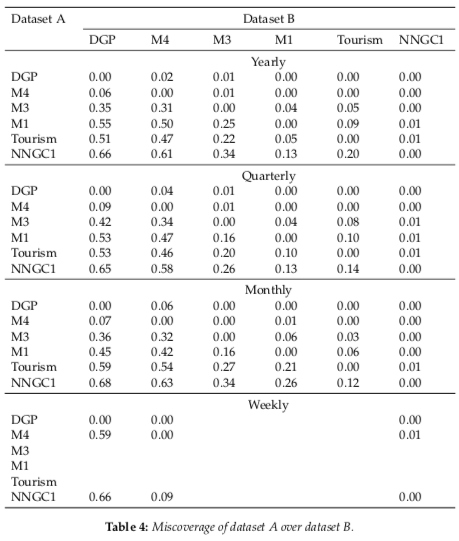
\includegraphics[height=\textheight]{figures/miscoverage.png}}

\end{frame}

\section{Extension to multiple seasonal time
  series}\label{extension-to-multiple-seasonal-time-series}

\begin{frame}{Simulation of multiple seasonal time series}

  \centerline{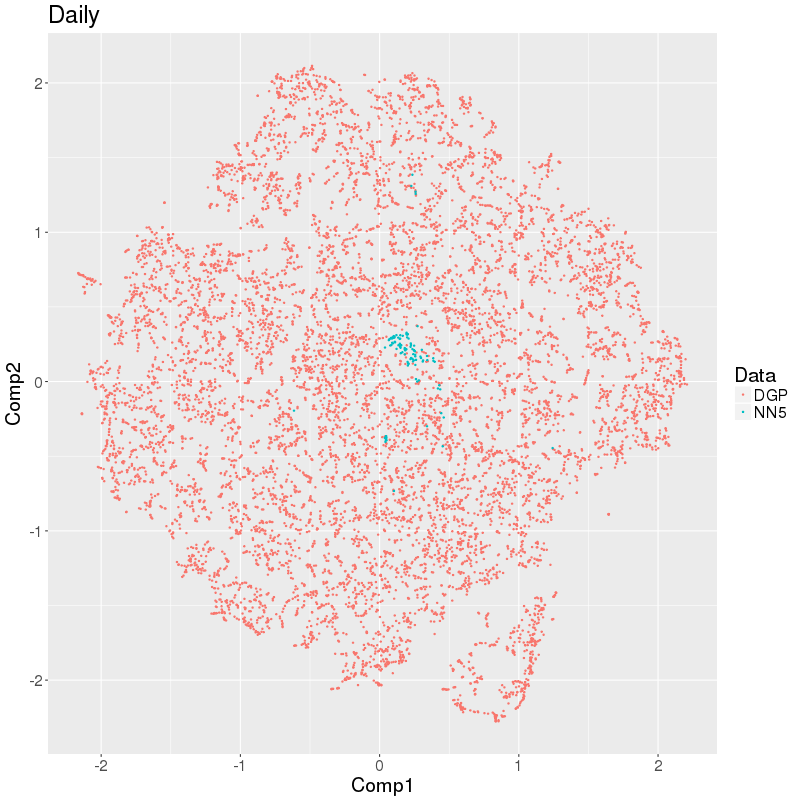
\includegraphics[width=0.6\textwidth]{figures/daily.png}}

\end{frame}

\section{New time series generation based on MAR
  models}\label{new-time-series-generation-based-on-mar-models}

\begin{frame}{New time series generation}

  \begin{itemize}
  \item
    Time series \(\rightarrow\) features \checkmark
  \item
    Time series \(\leftarrow\) features ?

    \begin{itemize}
      \tightlist
    \item
      Genetic Algorithm (GA) to evolve time series with length n
    \item
      GA to tune the MAR model parameters \(\Theta = (\alpha_k, \phi_i)\)
    \end{itemize}
  \end{itemize}

\end{frame}

\begin{frame}{GA procedure}

  \begin{itemize}
    \tightlist
  \item
    Firstly decide on the period \(P\) and length \(n\).
  \item
    Given a target \(T_i\) in the feature space. Find \(\Theta^{*}\) that
    can simulate \(X_{T_i}\) with its feature vector \(T_i\).
  \item
    Generate an initial population of size \(N_P\) for the parameter
    vector \(\Theta\) from the entire possible ranges.
  \item
    For each iteration, repeat the steps below.

    \begin{enumerate}
      \def\labelenumi{\arabic{enumi}.}
      \tightlist
    \item
      For each member in the current population, simulate a time series
      \(j\) and calculate its feature vector \(F_j\).
    \item
      Calculate the fitness value for each member:
      \[\text{Fitness}(j) = - ||F_j-T_i||.\]
    \item
      Produce the new generation based on the crossover, mutation and the
      survival.
    \end{enumerate}
  \item
    Upon convergence, we keep the cloest time series.
  \end{itemize}



\end{frame}

\begin{frame}{}

  \centerline{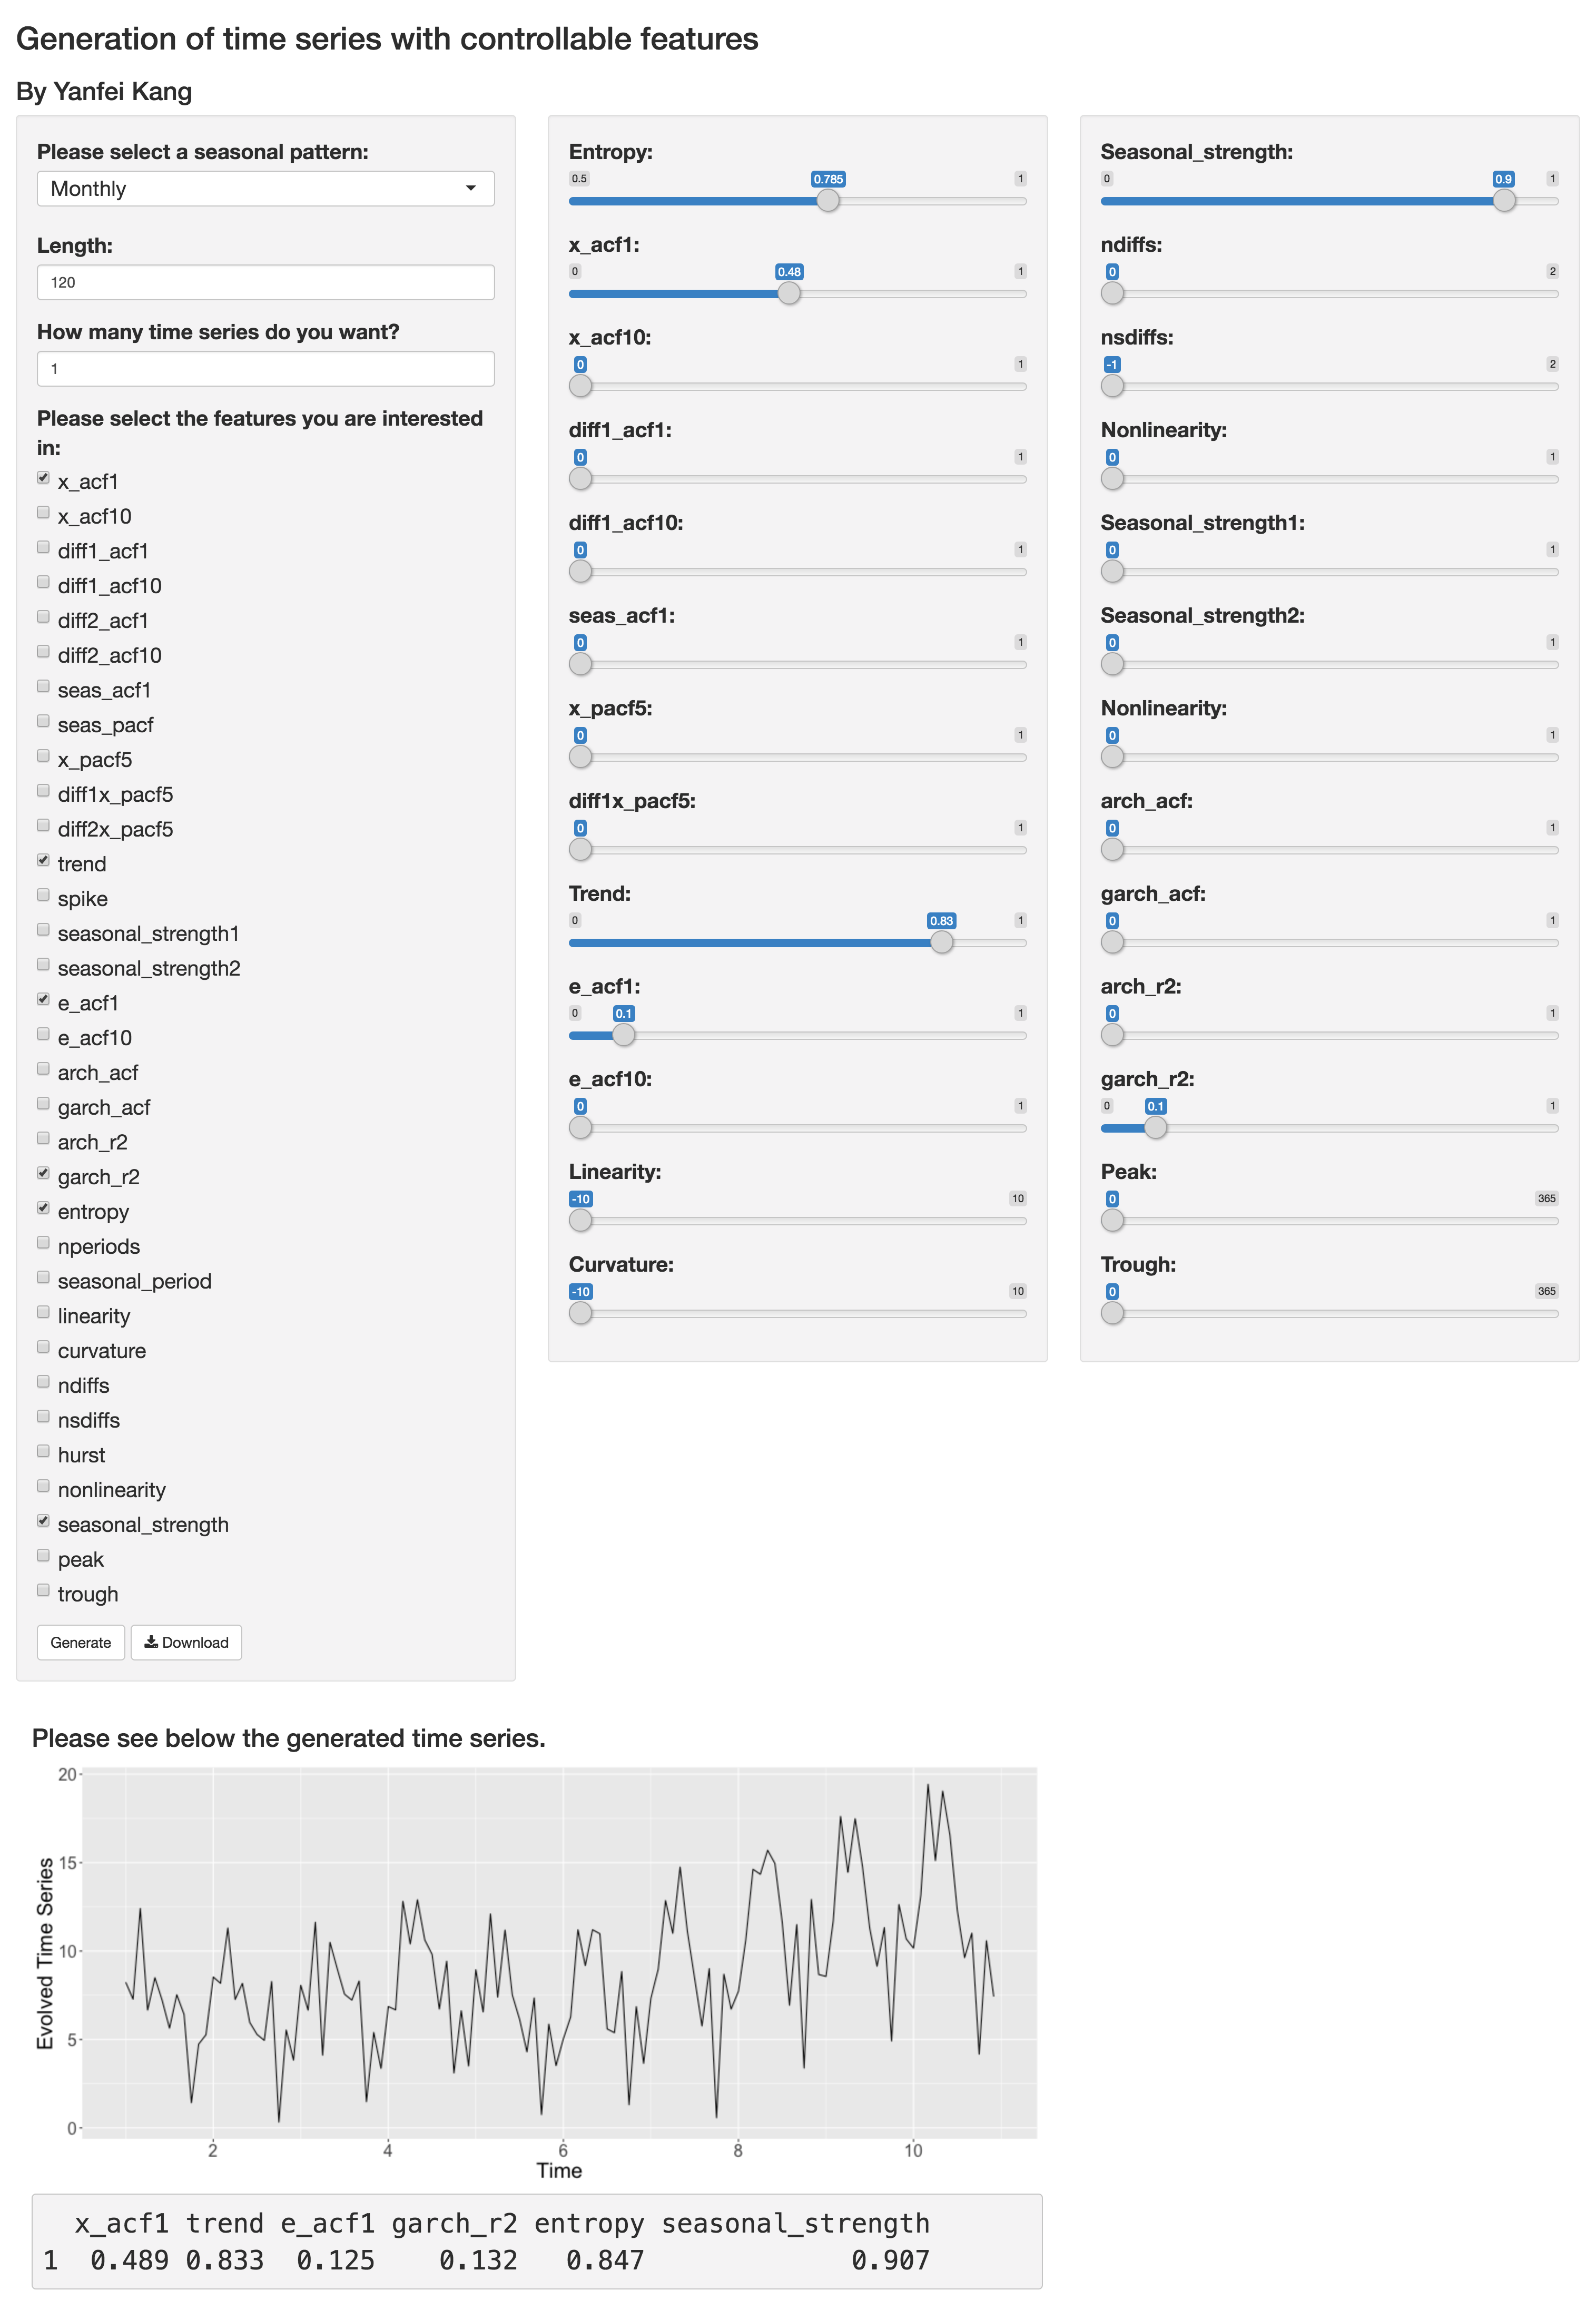
\includegraphics[height=0.8\textheight]{figures/TSgenerationApp}}

    \begin{itemize}
  \item R package: {\color{blue}\texttt{tsgeneration}} {\footnotesize available on GitHub \url{https://github.com/ykang/tsgeneration}}
  \end{itemize}

\end{frame}

\section{Forecasting based on features}\label{forecasting-based-on-features}

\begin{frame}{Time series forecasting methods}

  \metroset{block=fill}

  \begin{alertblock}{The six popular forecasting methods in time series}
    \begin{enumerate}
    \item Naïve: using the most recent observation as the forecast.
    \item Seasonal naïve: forecasts are equal to the most recent observation from the corresponding time of year.
    \item The Theta method, which performed particularly well in the M3-Competition.
    \item ETS: exponential smoothing state space modelling.
    \item ARIMA: autoregressive integrated moving average models.
    \item STL-AR: an AR model is fitted to the seasonally adjusted series, while the seasonal component is forecast using Seasonal naïve.
    \end{enumerate}
  \end{alertblock}

\end{frame}

\begin{frame}{Modelling features and forecasting performances on
    training data}

  \[\bf{MASE}_{N\times6} \Leftrightarrow \bf{F}_{N\times p}\]

  \[\mathbf{MASE^{(i)}} = f_1^{(i)}(F_1) + f_2^{(i)}(F2) + ... + f_p^{(i)}(F_p) + \epsilon^{(i)}\]
  \begin{itemize}
  \item This relationship is obviously nonlinear. We use the Bayesian spline regressions
    to capture the nonlinearity \citep{li2013efficient}.

  \item R package: {\color{blue}\texttt{movingknots}} {\footnotesize available on GitHub
      \url{https://github.com/feng-li/movingknots}}

  \end{itemize}

\end{frame}

\begin{frame}{Apply the model on the forecasts on M3 \\(out-of-sample)}

  \centerline{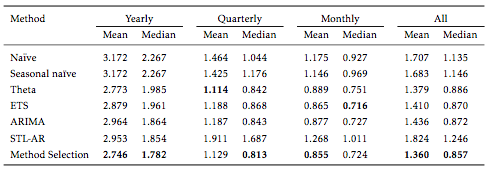
\includegraphics[height=\textheight]{figures/M3MASE.pdf}}

\end{frame}

\begin{frame}{Conclusions}

  \begin{itemize}
    \tightlist
  \item
    Feature description.
  \item
    Time series simulation from MAR models.
  \item
    2D space (identify unusual time series, find clusters, etc.).
  \item
    Develop meta-forecasting algorithms which choose a specific method
    based on the location of a time series in the instance space.
  \item
    Generate new time series with specific features.
  \end{itemize}

\end{frame}

\begin{frame}{Working in progress}

  \begin{itemize}
    \tightlist
  \item Extension to multivariate time series.

  \item Density forecasting.

  \item Framework on non-time series.

  \end{itemize}

\end{frame}


\begin{frame}[allowframebreaks,plain]%{References}
  \tiny
  \bibliography{MARpaper, References, full}
  \bibliographystyle{asa}
\end{frame}



\begin{frame}{Thanks!}

  \Large \texttt{\url{http://feng.li/}}

  \Large \texttt{\url{feng.li@cufe.edu.cn}}

\end{frame}

\end{document}
